\documentclass[]{article}
\usepackage{vmlmacros}
\usepackage{syntax}
\usepackage{relsize}
% \usepackage{palatino} % I don't love this, to be honest. 
\usepackage{amsmath}
\usepackage{booktabs}
\usepackage{simplebnf}
\usepackage{tikz}
\usepackage{float}
\floatstyle{boxed} 
\restylefloat{figure}

\setcounter{secnumdepth}{1}

\DeclareMathOperator{\dom}{dom}



% \setlength{\grammarparsep}{20pt plus 1pt minus 1pt} % increase separation between rules
\setlength{\grammarindent}{10em} % increase separation between LHS/RHS
\setlength{\parindent}{0cm}
\title{Syntax and Semantics of $V^{-}, P^{+}, and D$}
\author{Roger Burtonpatel}
\date{December 3, 2023}
\begin{document}

\maketitle

\section{Syntax}

\subsection{The Core Language}

We present a grammar of a base language, with no decision-making constructs: 

\bigskip

% I attempted to use the grammar environment you provided. But there was either
% something missing or something I overlooked in the example code and it would
% not compile, despite many reducing changes I made. So I went with the
% simplebnf package, which I quite like.  
\begin{center}
    \begin{bnf}
    $P$ : \textsf{Programs} ::=
    $\bracketed{d}$ : definition
    ;;
    $d$ : \textsf{Definitions} ::=
    | $\tt{val} \; x \; \tt{=} \; \expr$ : bind name to expression
    ;;
    $\expr$ : Core expressions ::= 
    | $x, y, z$ : names
    | $K\bracketed{\expr}$ : value constructor application 
    | $\tt{if} \; \expr[1] \; \tt{then} \; \expr[2] \; \tt{else} \; e_{3} $ : if
    | $\lambda x. \; \expr$ : lambda 
    | $\expr[1] \; \expr[2]$ : function application 
    ;;
    $v$ : Values ::= $K\bracketed{v}$ : value constructor application 
    ;;
    $K$ : \textsf{Value Constructors} ::=
    % \cons : cons 
    % | \tt{[]} : empty list 
    | \tt{true} $\vert$ \tt{false} : booleans
    | $\tt{\#}x$ : name beginning with \tt{\#}
    | \tt{A-Z}$x$ : name beggining with capital letter
    | $[\tt{-}\vert\tt{+}](\tt{0}-\tt{9})+$ : signed integer literal 

    \end{bnf}
\end{center}


A \it{name} is any token that is not an integer literal, 
does not contain whitespace, a bracket, or parenthesis, 
and is not a value constructor name or a reserved word.


We then present three languages that build off of this core: 
\Pplus, the language of patterns, \Vminus, the language of 
verse-like equations, and $D$, the language of decision trees. 

\subsection{Three Language Extensions}

\subsubsection{\Vminus:}

\begin{center}
    \begin{bnf}
    $\ealpha$ : \textsf{$\alpha$-Expressions} ::=
    | $x, y, z$ : names
    % Question: ebnf braces vs. 
    | $\tt{if} \; \tt{[}\; \galpha \; \bracketed{[] \galpha} \;\tt{]} \; \tt{fi}$ : if-fi 
    | $K \bracketed{\ealpha}$ : value constructor application 
    | $\ealpha[1] \; \ealpha[2]$ : function application 
    ;;
    $\galpha$ : \textsf{Guarded Expressions} ::=  
    $\boldsymbol{\rightarrow}\alpha$ : terminating $\alpha$ 
    | $\expr; \; \galpha$ : intermediate core expression 
    | $\exists \bracketed{x} \tt{.} \galpha$ : existential 
    | $\ealpha[1] = \ealpha[2]; \; \galpha$ : equation 
    % ;;
    \end{bnf}
\end{center}

\bigskip 

\subsubsection{\Pplus:}
\begin{center}
    \begin{bnf}
$\expr$ : \textsf{Expressions} ::=
    | $\ttbraced{\tt{case} \; \expr \; \bracketed{\tt{[} p \; \expr \tt{]}}}$ : case expression 
    ;;
    $p$ : \textsf{Patterns} ::= $x$ : name 
    | $K$ : value constructor 
    | $\ttbraced{K \; \bracketed{p}}$ : value constructor application 
    % | $\ttbraced{p \; \tt{when} \; \expr }$ : side condition
    | $\ttbraced{\tt{oneof} \; p_{1} \;, p_{2} }$ : or-pattern 
    | $\ttbraced{p \tt{;} \bracketed{\expr \vert \ttbraced{p  <- \expr}}}$ : pattern guard
    \end{bnf}
\end{center}


\bigskip 

\subsubsection{$D$:}

\begin{center}
    \begin{bnf}
        \Dalpha : \textsf{Decision Tree} ::= 
        $\tt{case} \; x \; \tt{of} \; 
        \bracketed{\vert \; K\bracketed{x} \; \tt{=>} \; \Dalpha}
        [\vert \; x \; \tt{=>} \Dalpha]$ : test node 
        | $\alpha$ : match node 
        | $\tt{if} \; x \; \tt{then} \; \Dalpha \; \tt{else} \; \Dalpha$ : condition with two children 
        | $\tt{let} \; x \; \tt{=} \; \expr \; \tt{in} \; \Dalpha$ : let-bind a name
        ;;
        $\expr$ : \textsf{Expressions} ::=
        | $\mathcal{D}_{\expr}$ : decision trees 
    \end{bnf}
\end{center}

\bigskip
\begin{figure}[H]
    \centering
    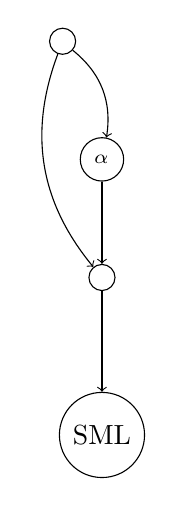
\begin{tikzpicture}
        \node[circle, draw] (1) at (5,5) {\Pplus};
        \node[circle, draw] (2) at (5.5,3.5) {$\Vminus_{\alpha}$};
        \node[circle, draw] (3) at (5.5,2) {\Dalpha};
        \node[circle, draw] (4) at (5.5,0) {SML};


        \draw[->] (1)[bend left] to (2);
        \draw[->] (2) to (3);
        \draw[->] (3) to (4);
        \draw[->] (1) to[bend right] (3);
    \end{tikzpicture}
    \caption{Flow of language translation.}
    \label{fig:graph}
\end{figure}

\section{The Three Languages}

The first of our languages is \Pplus. This is the language of patterns. We know
we can compile patterns into decision trees. Our next language is \Vminus, the
language of equations. This uses the decision making construct \it{if-fi} to
perform different operations based on the form of a value. 

Both of these languages theoretically can be compiled to our third language,
\D: the language of decision trees. 

\bigskip

\section{Language Structure}

The three langauges look similar: they each have value constructors and 
a 'decision-making construct' to deal with constructed data. In \Pplus, the 
construct is pattern-matching; in \Vminus, it is the guarded expression; 
in \D, it is the decision tree. 

Of note in both \Vminus and \D is that the 'decision-making construct' is 
annotated with an $\alpha$. This annotation gives us type flexibility on the 
right-hand side of the \it{terminating} case for each construct 
(\tt{$\rightarrow$ exp} in \Vminus and the match node in \D.) 

Because of the $\alpha$, the right-hand side becomes immaterial: we don't care
about what we're returning; we care about the decision-making construct that
gets us there. Whether it's a single value (ML-style) a sequence of values
(Verse-style), or even something else, the $\alpha$ represents \it{any} ultimate
result of "making a decision," and it's the ways in which we make decisions that
we truly care about examining. By making the return result both polymorphic and
abstract, we eschew the need to worry about its type and compatibility with
other results of otherwise-equivalent trees. 

\section{Translation and Equivalency}

We aim to translate $\Pplus$ to both $\Vminus$ and $\D$ (Figure 1). By showing both
languages can be translated to decision trees, we show both express a common
property: that evaluation at runtime does not backtrack, i.\expr., no individual
part of a value used to make decisions (called a \tt{scrutinee}) is examined
more than once. Showing \Vminus expresses this no-backtracking property (and, by
extension, the "no-logical-variables-at-runtime" property, is a core aim of this
work.)

The second important translation is from $\Vminus$ to \D. Recall the $\alpha$ from
earlier: the polymorphic abstract type in both $\galpha$ and $\Dalpha$ shows
an equivalence preserved by translation. 

\it{Rough- want to hack this out with you:} \\
The equivalence is this: final, returned right-hand sides of 'decision-making 
constructs' can be anything. 


        
\section{Refinement ordering on environments}

\begin{align*}
\rho \subseteq \rho' \text{ when }&\dom\rho  \subseteq \dom \rho'\\
\text{ and } &\forall x \in \dom \rho: \rho(x) \subseteq \rho'(x)
\end{align*}



\vfilbreak



\section{Forms of Judgement for $V^{-}$:}
\begin{tabular}{ll}
\toprule
    \multicolumn2{l}{\emph{Metavariables}} \\
\midrule
    % $v, \; v'$& value \\
    \valpha& a value produced from evaluating $\alpha$. \\
    $eq$& equation \\ 
    % $\tempstuck$& a temporarily-stuck equation \\
    $\reject$& equation rejection \\
    $\result$& $\vartheta \mid$ \reject : a result of \valpha \; or
    rejection\\
    $\rho$& environment: $name \rightarrow \mathcal{V}_{\bot}$ \\
    $\rho\{ x \mapsto y \} $& environment extended with name $x$ mapping to $y$ \\
    $\mathcal{T}$& Context of all temporarily stuck equations (a sequence) \\ 
    $\ealpha$& An expression \\ 
    $\galpha$& A guarded expression \\
    \uppsidown& Inability to compile to a decision tree; a compile time error \\
\bottomrule
\end{tabular}    

\bigskip

\begin{tabular}{ll}
    \toprule
        \multicolumn2{l}{\emph{Sequences}} \\
    \midrule
        $\emptyseq$& the empty sequence \\
        $S_1 \cdot S_2 $&  Concatenate sequence $S_1$ and sequence $S_2$ \\
        $x \cdot S_2 $& Cons $x$ onto sequence $S_2$ \\
    \bottomrule
    \end{tabular}    
    
    \medskip
    
    % \mkjudgementcmd{EquationSuccess}{\vtuple{\rho, eq}}{\rhohat REMOVE THIS}
    % \mkjudgementcmd{EquationTempStuck}{\vtuple{\rho, eq}}{\tempstuck}
    % \mkjudgementcmd{EquationReject}{\vtuple{\rho, eq}}{reject}

    % \showvjudgement{EquationSuccess}{\EquationSuccess}
    % \showvjudgement{EquationTempStuck}{\EquationTempStuck}
    % \showvjudgement{EquationReject}{\EquationReject}
    
    
    
    
    % Success only refines the environment; that~is, when
    % ${\vtuple{\rho, \expr}} \rightarrowtail{} {\rho'}$, we~expect $\rho \subseteq \rho'$.
    
    
\subsection{Expressions}

    \newcommand\EvalE{\vmrun[term=\alpha]}
    \newcommand\EvalGe{\vmrun}
    \newcommand\GNoTree{\vmrun \rightsquigarrow \uppsidown} An expression
    in core Verse evaluates to produce possibly-empty sequence of values. In
    \Vminus, values depend on the form of abstract expression $\alpha.$ If
    $\alpha$ is a Verse-like expression, \valpha will be a value sequence. If it
    is an ML-like expression, it will be a single value. 

    A guarded expression evaluates to produce a \bf{result}. A result is either
    a possibly-empty sequence of values or reject. 

    \[\it{r} \; \rm{::=} \; \vartheta \;|\; \reject \]

    \showvjudgement{Eval-Expr}{\EvalE}
    \showvjudgement{Eval-Guarded-Expr}{\EvalGe}
    
    \bigskip
    If a guarded expression cannot be evaluated without producing logical 
    variables at runtime, it cannot be expressed as a decision tree. 
    This notation indicates this failure (think of \uppsidown as a fallen 
    tree), which results in a compile-time error. 
    \showvjudgement{NoTree}{\GNoTree}

\bigskip


\section{Sequences}

The trivial sequence is \emptyseq. Sequences can be concatenated with infix 
$\cdot$. In an appropriate context, a value like $x$ stands for 
the singleton sequence containing $x$. 

\begin{align*}
    \emptyseq \cdot \ys &\equiv \ys \\
    \ys \cdot \emptyseq &\equiv \ys \\
    (\xs \cdot \ys) \cdot \zs &\equiv \xs \cdot (\ys \cdot \zs)
\end{align*}

\section{Rules (Big-step Operational Semantics) for $V^{-}$:}
    
\subsection{Evaluating Guarded Expressions}
\subsubsection{Evaluating simple parts of guarded expressions}

\[
\inferrule*[Left=\textsc{ (Eval-ArrowExpr) }]
    {\vmrun[context=\emptyseq,term=\alpha,result=\vartheta]}
    {\vmrun[context=\emptyseq, term=\rightarrow \alpha,result=\vartheta]}
\]

\[
\inferrule*[Left=\textsc{ (Eval-Exists) }]
    {\vmrun[env=\rho\{x \mapsto \bot \}]}
    {\vmrun[term=\exists x.\; \galpha]}
\]

\[
\inferrule*[Left=\textsc{ (Eval-Expseq) }]
    {\inferrule* {}
    {
    \veval{\ealpha}{\valpha}
    \and
    \veval{\galpha}{\result}
    }}
    {\vmrun[term=\ealpha;\; \galpha]}
\]
\subsubsection{Shifting an equation to the context}
\[
\inferrule*[Left=\textsc{ (G-Move-To-Ctx) }]
    {\inferrule*{\vmrun[context=eq \cdot \context]}
    {}
    }
    {\vmrun[term=eq; \; \galpha]}
\]

\subsubsection{Evaluating with different types of equations}

\[
\inferrule*[Left=\textsc{ (G-EqExps) }]
    {\inferrule* {}
    {
    x,\;y \; \rm{are distinct and fresh}
    \\\\
    \vmrun[envext=\bracketed{x \mapsto \bot,\; y \mapsto \bot},
          context=\eqTT{x = \ealpha[1] \cdot y = \ealpha[2] \cdot x = y}]}}
    {\vmrun[context=\TeqT{\ealpha[1] = \ealpha[2]}]}
\]

\[
\inferrule*[Left=\textsc{ (G-EqNameExp) }]
    {\inferrule* {}
    {
    \veval{\ealpha}{\valpha}
    \and 
    \vmrun[envext=\bracketed{x \mapsto \valpha},
           context=\context \cdot \context',result=\result']}}
    {\vmrun[context=\TeqT{x = \ealpha},result=\result']}
\]

\[
\inferrule*[Left=\textsc{ (G-EqNames-Vals-Succ) }]
    {\inferrule* {}
    {
    x,\;y \in \dom \rho
    \\\\
    \rho(x) = \valpha, \; \rho(y) = \valpha
    \\\\ 
    \vmrun[context=\TT]}}
    {\vmrun[context=\TeqT{x = y}]}
\]

\[
\inferrule*[Left=\textsc{ (G-EqNames-Vals-Fail) }]
    {\inferrule* {}
    {
    x,\;y \in \dom \rho
    \\\\
    \rho(x) = \valpha, \; \rho(y) = \valpha'
    \\\\
    \valpha \neq \valpha'}}
    {\vmrun[context=\TeqT{x = y},result=\reject]}
\]

\[
\inferrule*[Left=\textsc{ (G-EqNames-Bots-Fail) }]
    {\inferrule* {}
    {
    x,\;y \in \dom \rho
    \\\\
    \rho(x) = \bot, \; \rho(y) = \bot
    \\\\
    x,\;y \; \rm{do not appear in} \; \context, \; \context'}}
    {\vmrun[context=\TeqT{x = y}] 
    \rightsquigarrow \uppsidown}
\]

\[
\inferrule*[Left=\textsc{ (G-EqNames-BotVal-Succ) }]
    {\inferrule* {}
    {
    x,\;y \in \dom \rho
    \\\\
    \rho(x) = \bot, \; \rho(y) = \valpha
    \\\\
    \vmrun[envext=\bracketed{x \mapsto \valpha},
           context=\context \cdot \context',result=\result']}}
    {\vmrun[context=\TeqT{x = y},result=\result']}
\]

\[
\inferrule*[Left=\textsc{ (G-Vcon-Single-Fail) }]
    {K \neq K'}
    {\vmrun[context=\TeqT{K = K'},result=\reject]}
\]

\[
\inferrule*[Left=\textsc{ (G-Vcon-Single-Succ) }]
    {\vmrun[context=\TT]}
    {\vmrun[context=\TeqT{K= K}]}
\]


\[
\inferrule*[Left=\textsc{ (G-Vcon-Multi-Fail) }]
    {K \neq K'}
    {\vmrun[context=\TeqT{K(\ealpha[1], \dots 
            \ealpha[n]) = K'(\ealpha[1]', \dots \ealpha[n]')},
            result=\reject]}
\]

\[
\inferrule*[Left=\textsc{ (G-Vcon-Multi-Arity-Fail) }]
    {n \neq m}
    {\vmrun[context=\TeqT{K(\ealpha[1], \dots 
            \ealpha[n]) = K(\ealpha[1]', \dots \ealpha[m]')},
            result=\reject]}
\]

\[
\inferrule*[Left=\textsc{ (G-Vcon-Multi-Succ) }]
    {
    \vmrun[context=\eqTT{\lbrack \ealpha[i]=\ealpha[i]' \; 
           \vert \; 1 \leq i \leq n \rbrack}]}
    {\vmrun[context=\TeqT{K(\ealpha[1], \dots 
            \ealpha[n]) = K(\ealpha[1]', \dots \ealpha[n]')}]}
\]

\subsection{Evaluating General Expressions}


% \[
% \inferrule*[Left=\textsc{ (If-Fi-Fail) }]
%     {\ }
%     {\veval{\iffi{\ }}{\emptyseq}}
% \]

\[
\inferrule*[Left=\textsc{ (If-Fi-Success) }]
    {\vmrun[] \Downarrow \vartheta}
    {\veval{\iffi{\galpha \; \square \; \dots}}{\vartheta}}
\]

\[
\inferrule*[Left=\textsc{ (If-Fi-Reject) }]
    {\inferrule* {}
    {\vmrun[result=\reject]}
    \and 
    \veval{\iffi{\dots}}{\vartheta}}
    {\veval{\iffi{\galpha \; \square \; \dots }}{\vartheta}}
\]

\[
\inferrule*[Left=\textsc{ (Vcon-Empty) }]
    {\ }
    {\veval{K}{K}}
\]

\[
\inferrule*[Left=\textsc{ (Vcon-Multi) }]
    {\inferrule* {}
    {
    \veval{\ealpha[i]}{\vartheta_{i}}
    \and 
    1 \leq i \leq n
    }}
    {\veval{K(\ealpha[1], \dots \ealpha[n])}{K(\vartheta_{1}, 
    \dots \vartheta_{i})}}
\]
\end{document}
